



\definecolor{menovagreen}{RGB}{230,245,230}
\definecolor{lightred}{RGB}{255,200,200}

\setcounter{secnumdepth}{4}

\chapter{Présentation générale du projet}
\minitoc
%\label{chap_biblio}

\section*{Introduction}
\addcontentsline{toc}{section}{Introduction}
Dans ce chapitre, nous commençons par présenter la société d’accueil dans laquelle s’est déroulé notre projet de fin d’études. Par la suite, nous analysons la situation actuelle afin de mettre en évidence les limites existantes, puis nous présentons la solution proposée, qui sera développée en détail dans les chapitres suivants. Enfin, nous terminons ce chapitre par la description de la méthodologie adoptée pour la conception du projet.

\section{Organisme d’accueil}
\subsection{Présentation de société}
Nous avons réalisé notre stage de fin d'études au sein de l'entreprise "SOTUPUB", spécialisée dans les services informatiques pour les entreprises. Elle propose une large gamme de presentations, allant de la fourniture et l'installation de systèmes informatiques à la maintenance, la sécurisation, la conception de sites web et d'applications, et le développement informatique sur mesure. SOTUPUB répond ainsi aux besoins croissants du marché numérique et assure un soutien continu à ses clients.

\begin{figure}[htpb]
    \centering
    
\includegraphics[width=6cm]{images/sotupub.png}
\end{figure}
\subsection{Les Services}
SOTUPUB se concentre sur huit domaines d'expertise clés :
\\
1. Installation et intégration de systèmes informatiques..
\\
2. Développement d’applications web et mobiles.
\\
3. Maintenance, sécurisation et support des systèmes informatiques.
\\
4. Infogérance et contrats de maintenance.
\\
5. Gestion et suivi du parc informatique.
\\
6. Vente et fourniture de matériel informatique.
\\
7. Accompagnement et conseil en développement informatique.
\\
8. Mise en œuvre de technologies innovantes et de pointe.

\section{Etude préalable}
\subsection{Contexte de projet}
Avec le développement rapide des technologies mobiles et de la géolocalisation, la sécurité des personnes vulnérables, notamment les enfants et les personnes âgées, est devenue un enjeu important. Malgré l’existence de certaines applications de suivi, celles-ci restent limitées et ne permettent pas une détection intelligente des situations à risque. Ainsi, il devient nécessaire de proposer une solution mobile fiable et sécurisée, capable d’assurer un suivi en temps réel et d’envoyer des alertes automatiques. C’est dans ce contexte que s’inscrit le projet SafeTrack, visant à renforcer la protection des personnes vulnérables grâce à une application intelligente.

\subsection{Problématique}


La sécurité des personnes vulnérables, telles que les enfants et les personnes âgées, représente un défi majeur dans la société actuelle. Malgré la disponibilité de certaines solutions de géolocalisation, celles-ci restent souvent limitées à un simple suivi de position, sans permettre une détection intelligente des situations à risque ni une intervention rapide en cas d’urgence. Cette absence de fonctionnalités avancées peut entraîner des retards d’alerte, une surveillance inefficace et une exposition accrue au danger. Il devient ainsi indispensable de concevoir une solution mobile centralisée, intelligente et sécurisée, capable d’assurer un suivi en temps réel, d’analyser les comportements et de faciliter une réaction immédiate afin de garantir une meilleure protection des personnes vulnérables.

      
\subsection{Étude de l’existant}
À ce jour, un certain nombre de solutions technologiques permettent le suivi de personnes en temps réel, la géolocalisation, la gestion d’alertes et la sécurité des utilisateurs, mais elles restent souvent spécifiques à un usage, sans proposer une solution globale et intelligente pour les personnes vulnérables comme le fait SafeTrack.

\subsubsection{FindMyKids \cite{findmykids}}

Application mobile de surveillance pour enfants qui permet de suivre leur géolocalisation en temps réel, de définir des zones sécurisées (geofencing) et de recevoir des alertes en cas d’urgence ou de dépassement de zone. Elle offre aussi un historique des mouvements et des notifications spécifiques pour assurer la sécurité des enfants.
\begin{figure}[htpb]
    \centering
    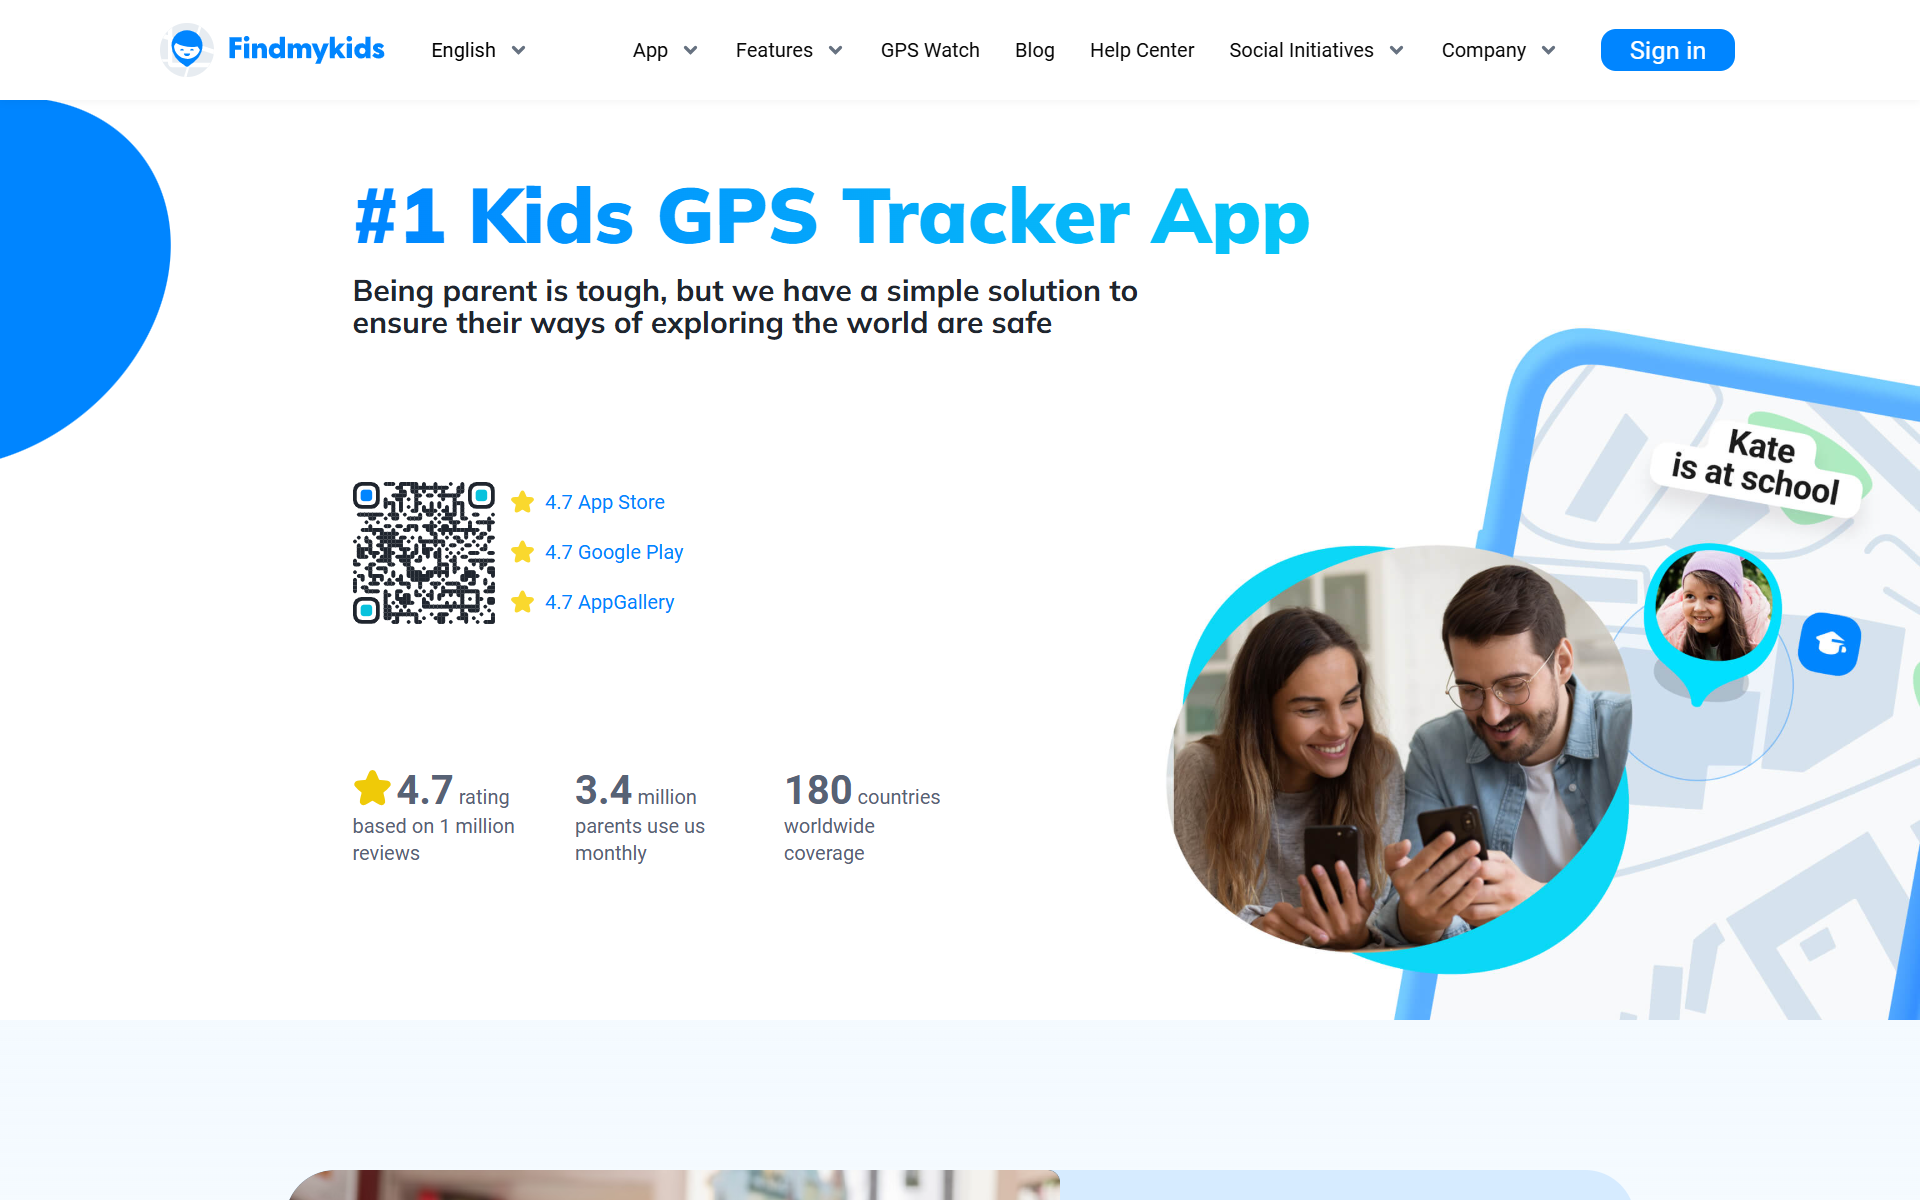
\includegraphics[width=10cm]{images/Capture d'écran 2026-02-04 121013.png}
    \caption{interface de Findmykids}
    \label{fig:findmykids}
\end{figure} 

\paragraph{Avantages :}
\begin{itemize}
    \item Géolocalisation en temps réel permettant aux parents de suivre les déplacements de l’enfant de manière continue.
    \item Fonctionnalité de zones sécurisées (geofencing) avec notifications automatiques en cas d’entrée ou de sortie d’une zone définie.
    \item Interface mobile simple et intuitive, facilitant la prise en main par les utilisateurs non techniques.
\end{itemize}

\paragraph{Inconvénients :}
\begin{itemize}
    \item Solution principalement orientée vers les enfants, avec une faible adaptabilité pour les personnes âgées ou atteintes de troubles cognitifs.
    \item Dépendance à une connexion Internet et à l’état de la batterie du smartphone, ce qui peut limiter la fiabilité en situation critique.
    \item Absence d’un système avancé d’analyse intelligente des comportements ou d’un dashboard web dédié aux organisations.
\end{itemize}

\subsubsection{MiniFinder \cite{minifinder}}

MiniFinder Nano / Pico / Watch est une solution de géolocalisation destinée à la sécurité des personnes vulnérables (enfants et personnes âgées). Elle offre un suivi en temps réel via des traceurs GPS et une application mobile ou web, avec des fonctionnalités comme le bouton SOS, le géorepérage et, selon le modèle, la détection de chute. Cependant, elle dépend d’un matériel dédié et propose peu de fonctionnalités d’analyse intelligente, limitant les possibilités de prévention avancée.

\begin{figure}[htpb]
    \centering
    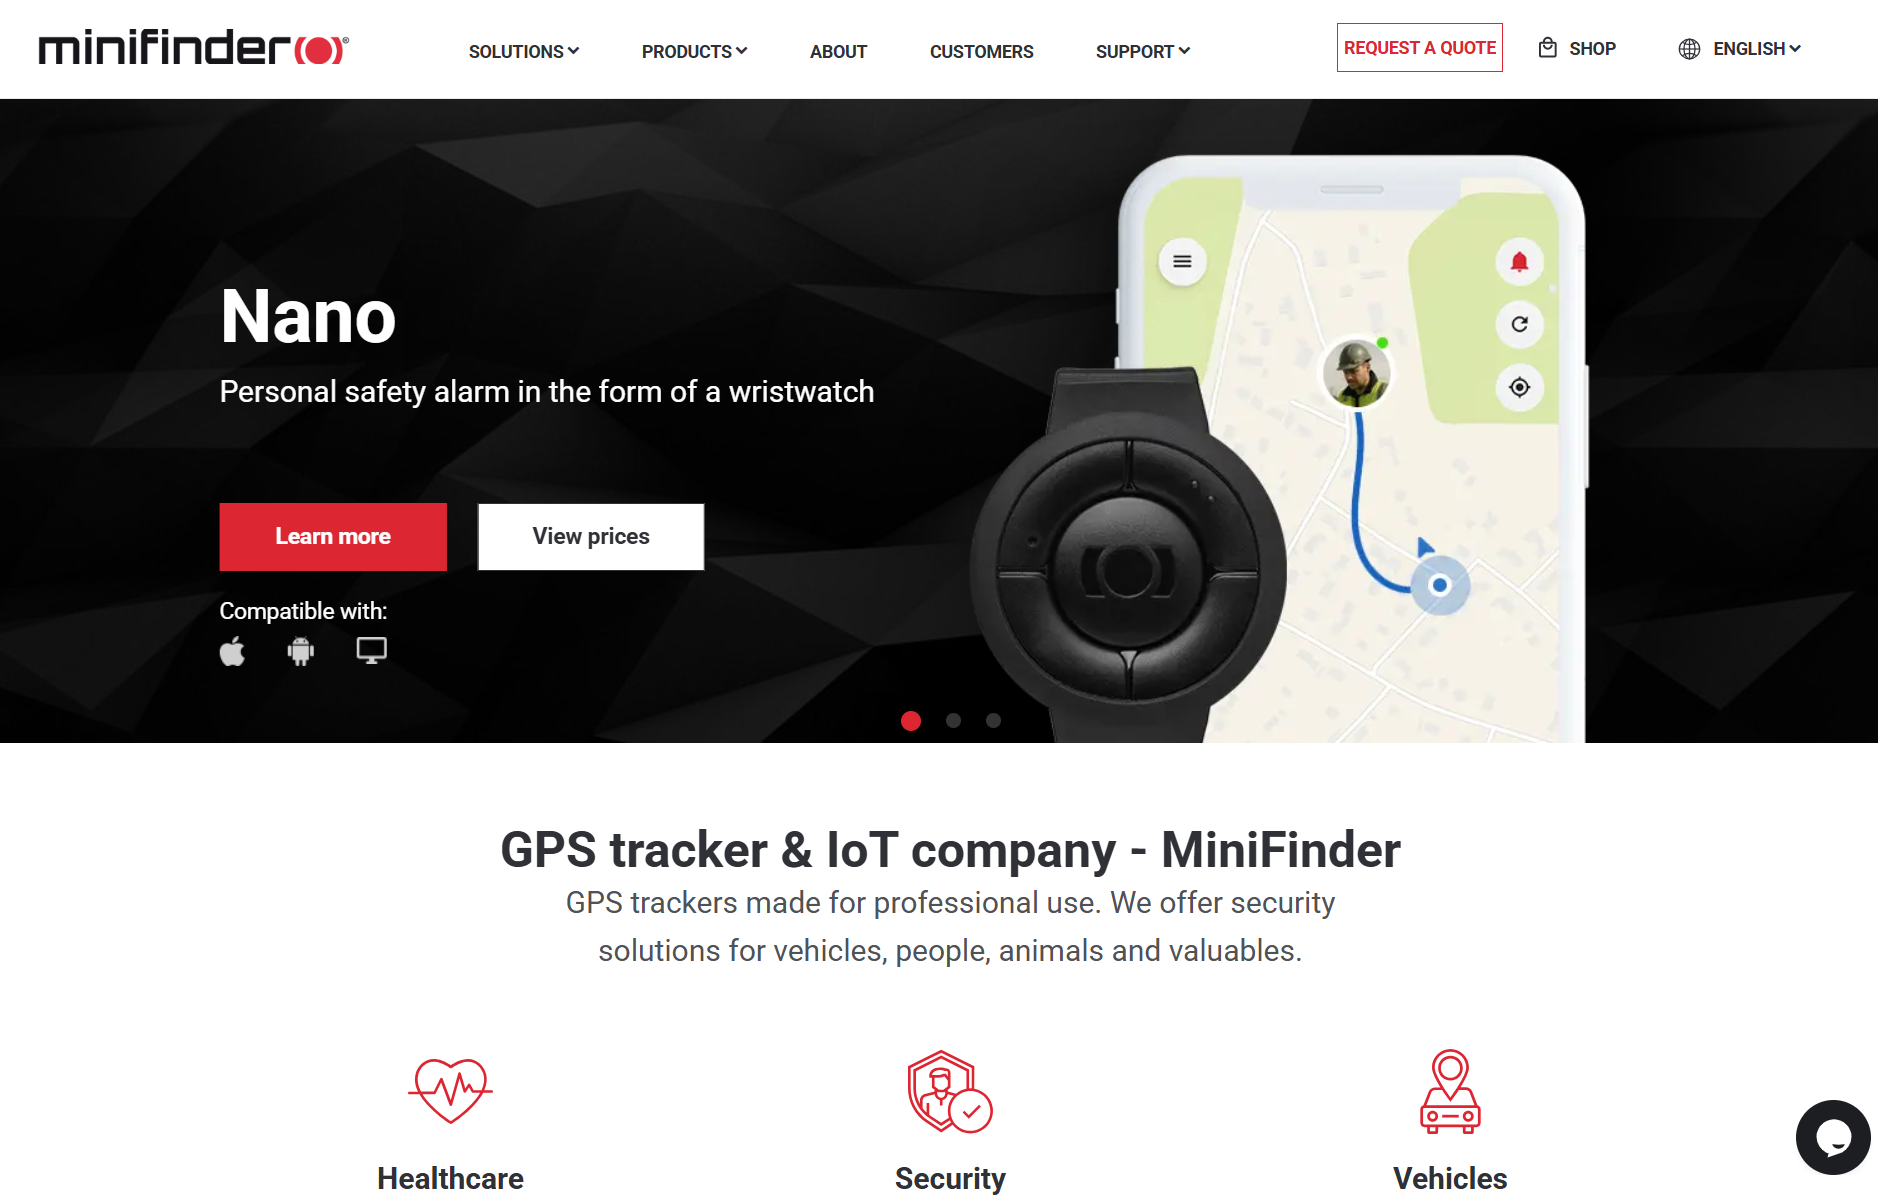
\includegraphics[width=10cm]{images/minifinderapp.png}
    \caption{Interface de Minifinder}
    \label{fig:teams}
\end{figure} 


\paragraph{Avantages :}
\begin{itemize}
    \item Géolocalisation en temps réel précise.
    \item Présence d’un bouton SOS pour les situations d’urgence.
    \item Utilisation simple, adaptée aux personnes vulnérables.
\end{itemize}

\paragraph{Inconvénients :}
\begin{itemize}
    \item  Dépendance à un dispositif matériel externe.
    \item Coût relativement élevé.
    \item Fonctionnalités d’intelligence artificielle limitées.
\end{itemize}

\subsubsection{Life360 \cite{life360}}

Application de suivi familial qui partage la position des membres en temps réel, facilite la communication entre eux et inclut des fonctionnalités de géorepérage. Elle est largement utilisée pour coordonner la sécurité des membres de la famille, notamment des enfants et des seniors.
\begin{figure}[htpb]
    \centering
    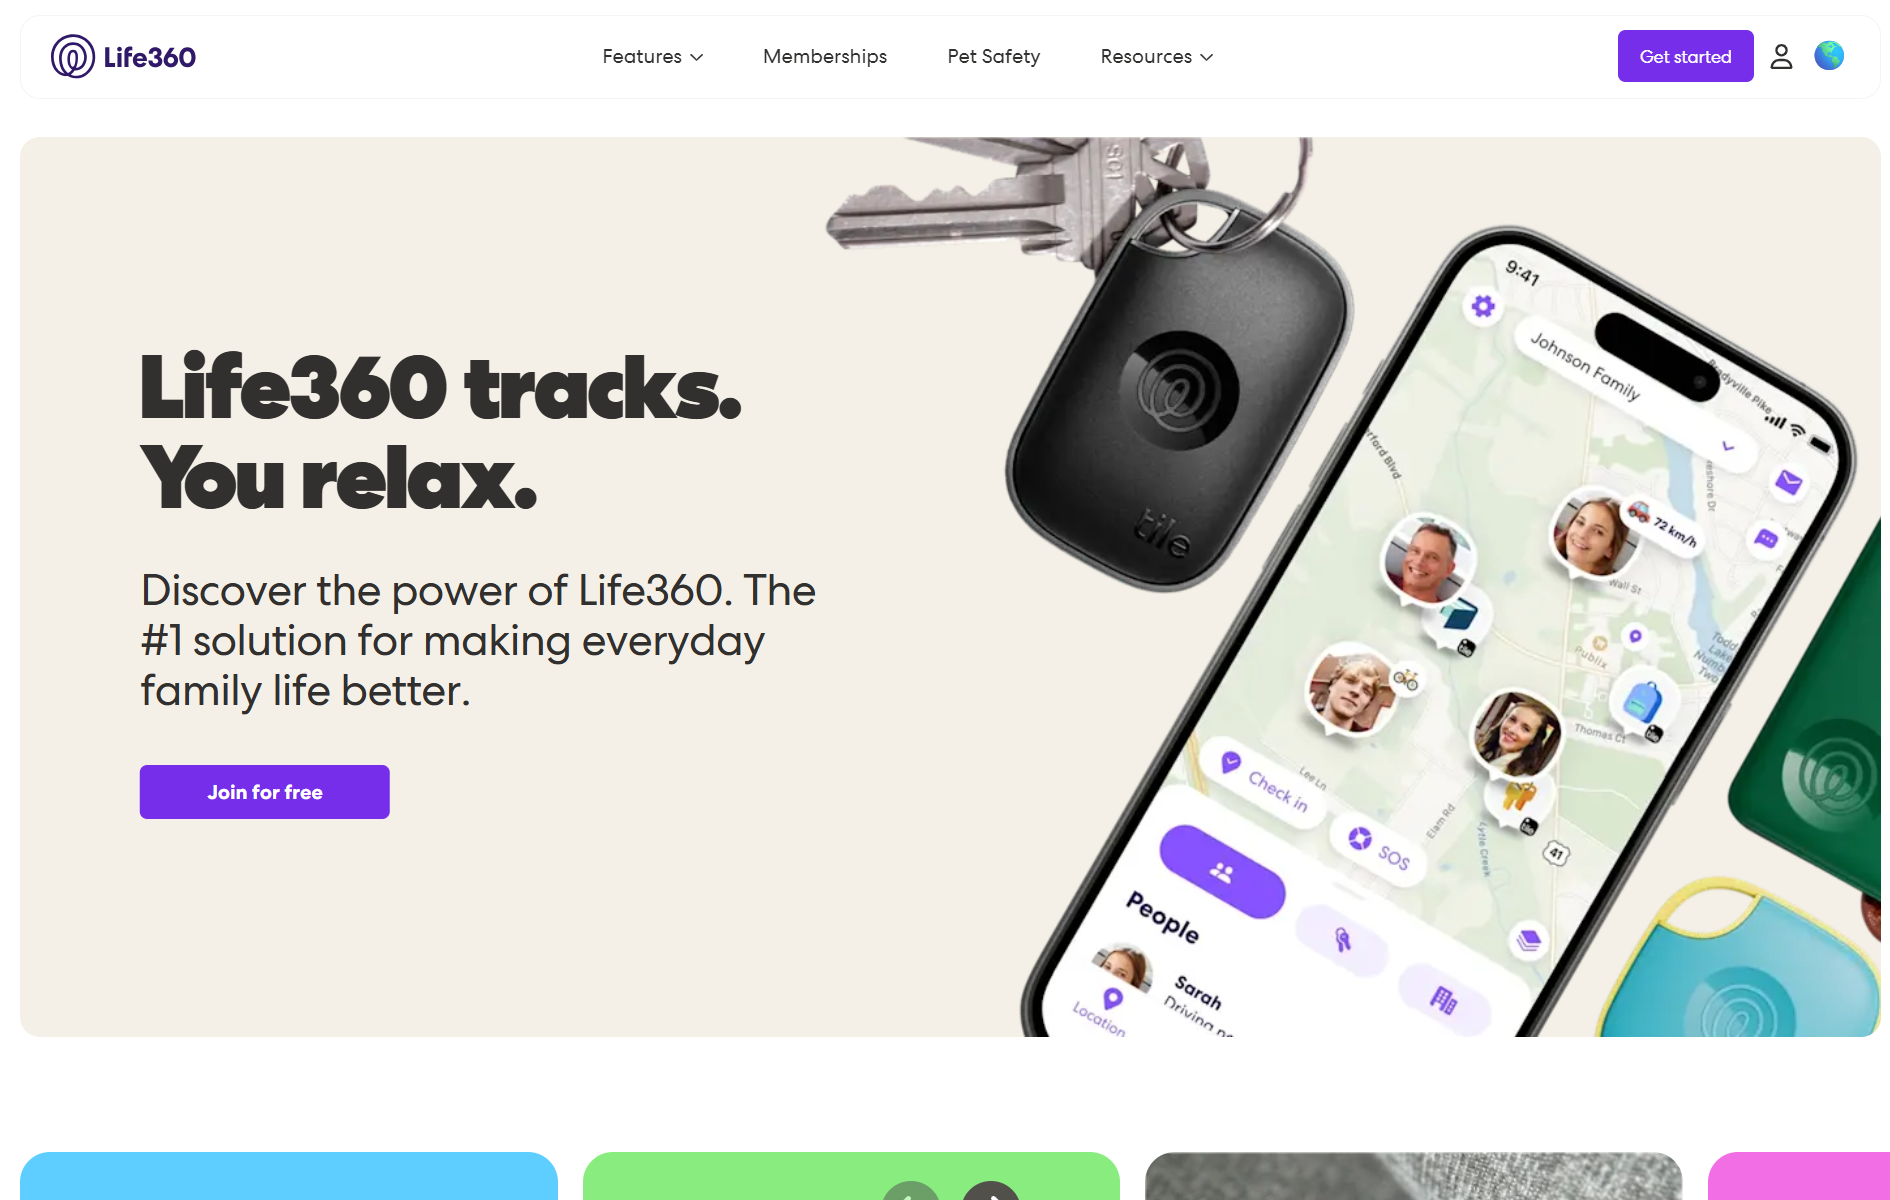
\includegraphics[width=10cm]{images/life360.png}
    \caption{Interface de Life360}
    \label{fig:life360}
\end{figure} 



\paragraph{Avantages :}
\begin{itemize}
    \item Géolocalisation en temps réel fiable permettant le suivi continu des membres d’un groupe familial.
    \item Fonctionnalité de géorepérage (geofencing) avec alertes automatiques lors de l’entrée ou de la sortie des zones définies.
    \item Intégration de fonctionnalités de communication et de notifications facilitant la coordination entre les membres.
\end{itemize}

\paragraph{Inconvénients :}
\begin{itemize}
    \item Application principalement orientée vers un usage familial, peu adaptée aux besoins des organisations ou des environnements professionnels.
    \item Absence de mécanismes avancés d’intelligence artificielle pour la détection automatique des comportements à risque.
    \item Fonctionnalités avancées souvent limitées à la version payante, ce qui peut représenter un frein à l’adoption.
\end{itemize}



\subsubsection{Mobile Tracker \cite{mobiletracker}}

Mobile Tracker est une application de géolocalisation permettant le suivi en temps réel des personnes vulnérables, avec des fonctionnalités de zones sécurisées et d’alertes d’urgence, visant à renforcer la sécurité des utilisateurs.


\begin{figure}[htpb]
    \centering
    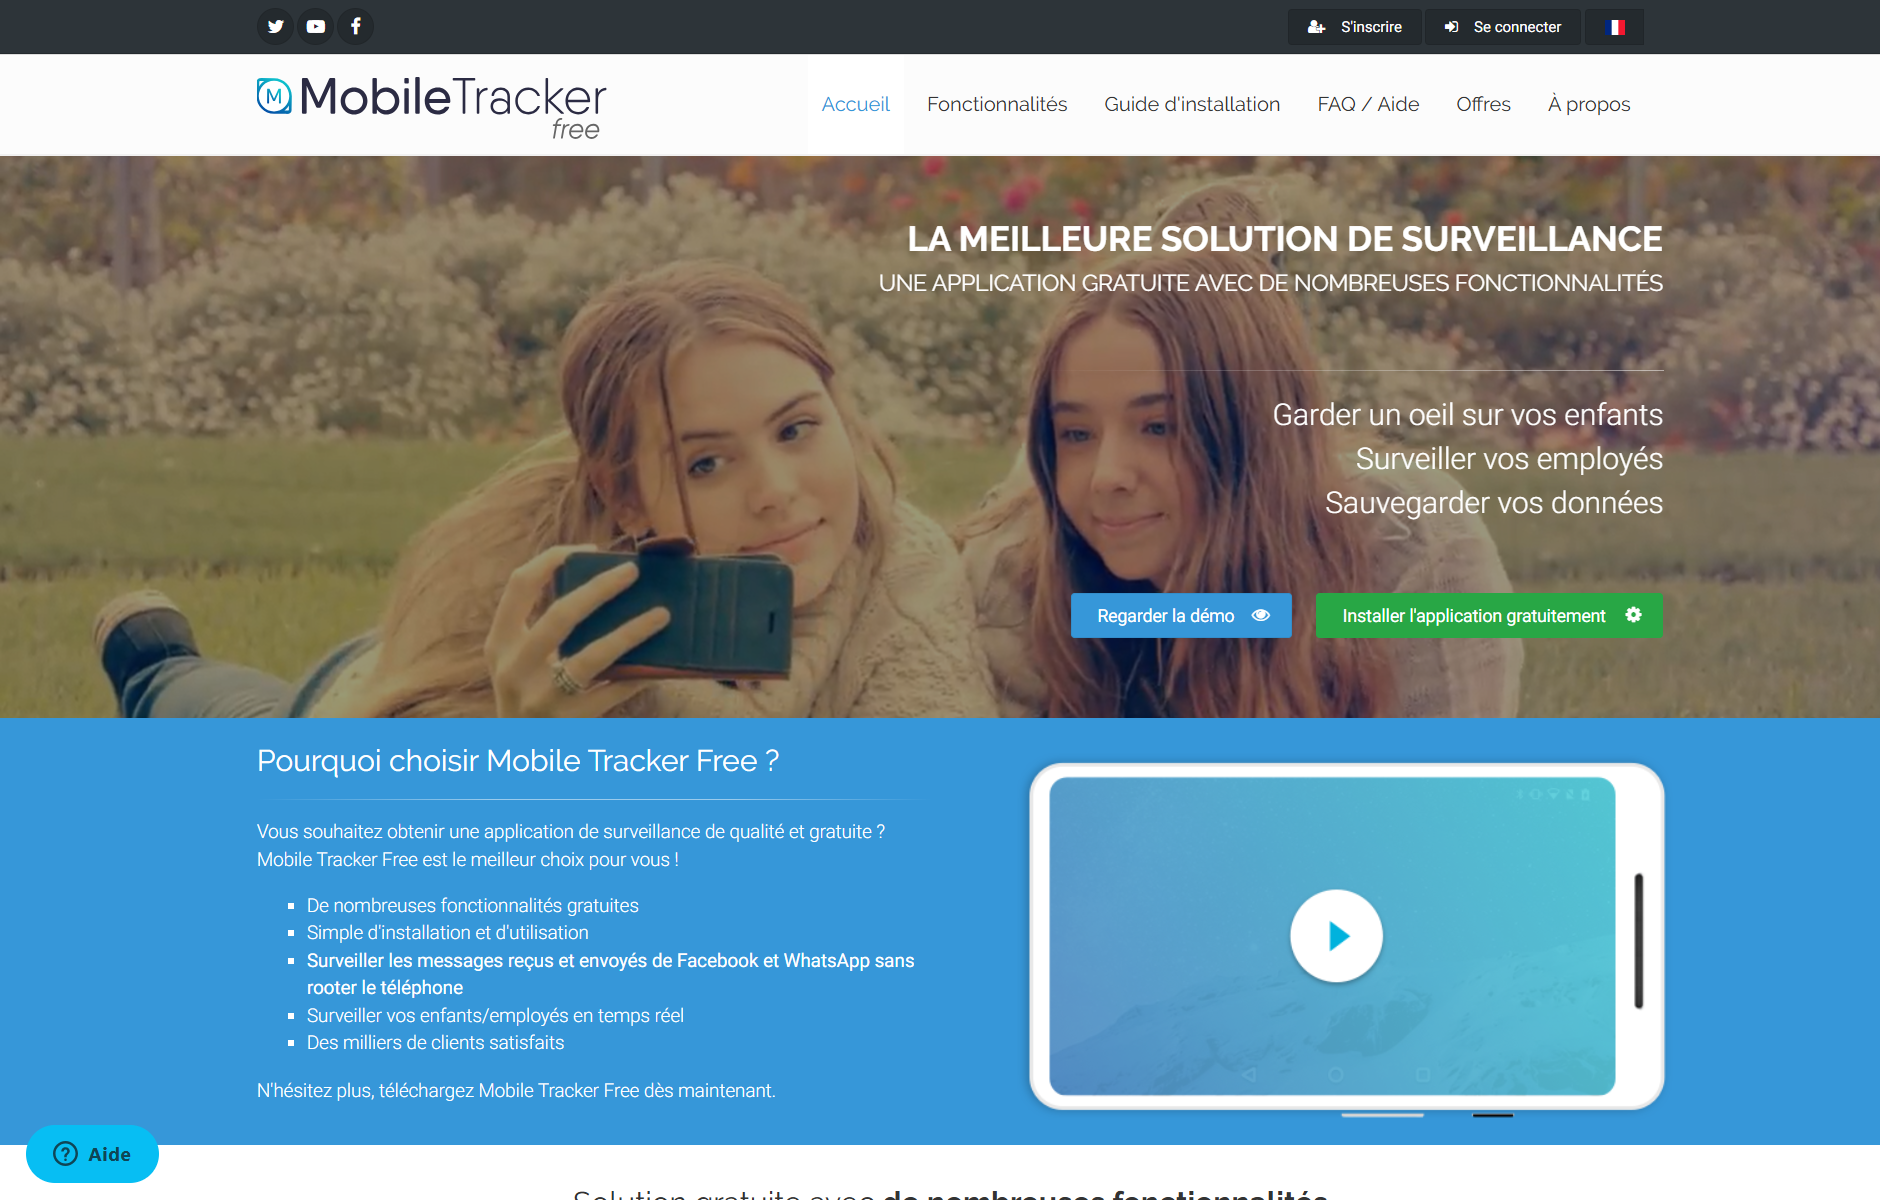
\includegraphics[width=10cm]{images/mobiletracker.png}
    \caption{Interface de Mobile Tracker}
    \label{fig:mobiletracker}
\end{figure} 



\paragraph{Avantages :}
\begin{itemize}
    \item Géolocalisation en temps réel permettant le suivi des déplacements des personnes vulnérables, notamment les personnes âgées.
    \item Mise en place de zones sécurisées avec alertes automatiques en cas de sortie des périmètres définis.
    \item Fonctionnalité de bouton SOS facilitant l’envoi rapide d’alertes en situation d’urgence.
\end{itemize}

\paragraph{Inconvénients :}
\begin{itemize}
    \item Interface et fonctionnalités souvent limitées, offrant peu de possibilités de personnalisation selon les profils des utilisateurs.
    \item Dépendance aux capteurs et à la connectivité du smartphone, ce qui peut réduire la fiabilité en cas de panne ou de faible batterie.
    \item Absence d’un tableau de bord web centralisé et de mécanismes intelligents d’analyse des comportements.
\end{itemize}



\subsubsection{FamiSafe \cite{famisafe}}
FamiSafe offre un suivi GPS en temps réel, la définition de zones sécurisées, et des alertes aux parents. Elle permet également de contrôler l’accès aux applications et de surveiller certaines activités numériques.



\begin{figure}[htpb]
    \centering
    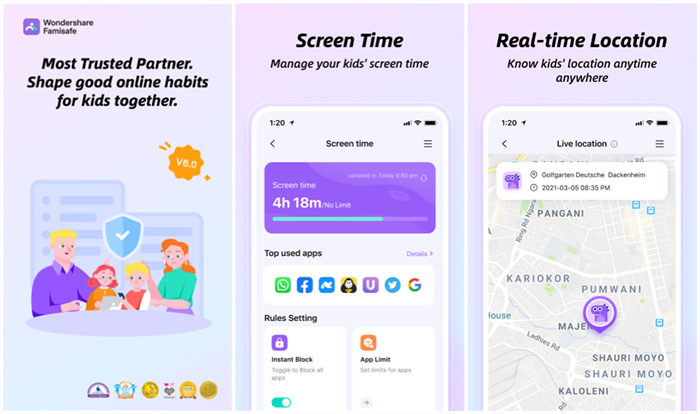
\includegraphics[width=10cm]{images/familesafe.jpg}
    \caption{Interface de mobile tracker famisafe}
    \label{fig:safeWatch}
\end{figure} 



\paragraph{Avantages :}
\begin{itemize}
    \item Combine suivi de localisation et contrôle des usages numériques dans une seule application.
    \item Permet de définir des zones géographiques avec notifications automatiques.
    \item Offre des outils de filtrage de contenus et de gestion des applications.
    
    
\end{itemize}

\paragraph{Inconvénients :}
\begin{itemize}
    \item Les fonctionnalités de sécurité physique restent basiques et non prédictives.
    \item Ne prend pas en charge la gestion scolaire ou le transport des enfants.
    \item Analyse limitée des comportements inhabituels.
   
\end{itemize}



\subsection{Étude comparative}
% Le tableau \ref{ref_tab_comp_existant} présente une étude comparative des solutions de suivi et de sécurité existantes.
Les différentes solutions de suivi et de géolocalisation des personnes vulnérables présentent des fonctionnalités intéressantes, mais restent souvent limitées ou spécialisées. SafeTrack se distingue par une approche globale en regroupant la géolocalisation en temps réel, la gestion des zones sécurisées, les alertes d’urgence et l’analyse intelligente des comportements au sein d’une seule plateforme. Cette intégration permet d’améliorer la prévention des risques, la réactivité en cas d’incident et l’efficacité du suivi.
\newpage


\begin{table}[ht]
    \centering
    \renewcommand{\arraystretch}{1.5}
    \resizebox{\textwidth}{!}{%
    \begin{tabular}{|l|m{3cm}|m{3cm}|m{3cm}|m{3cm}|m{3cm}|m{3cm}|}
        \hline
        \rowcolor{gray!20}
        \textbf{Critères} 
        & \textbf{SafeTrack} 
        & \textbf{FindMyKids} 
        & \textbf{Life360} 
        & \textbf{MiniFinder} 
        & \textbf{Mobile Tracker} 
        & \textbf{FamiSafe} \\
        \hline
        
        Géolocalisation en temps réel 
        & \cellcolor{green!20}$\checkmark$ 
        & \cellcolor{green!20}$\checkmark$ 
        & \cellcolor{green!20}$\checkmark$ 
        & \cellcolor{green!20}$\checkmark$ 
        & \cellcolor{green!20}$\checkmark$ 
        & \cellcolor{green!20}$\checkmark$ \\
        \hline

        Zones sécurisées (Geofencing) 
        & \cellcolor{green!20}$\checkmark$ 
        & \cellcolor{green!20}$\checkmark$ 
        & \cellcolor{green!20}$\checkmark$ 
        & \cellcolor{green!20}$\checkmark$ 
        & \cellcolor{green!20}$\checkmark$ 
        & \cellcolor{green!20}$\checkmark$ \\
        \hline

        Bouton SOS / alertes d'urgence 
        & \cellcolor{green!20}$\checkmark$ 
        & \cellcolor{green!20}$\checkmark$ 
        & \cellcolor{green!20}$\checkmark$ 
        & \cellcolor{green!20}$\checkmark$ 
        & \cellcolor{red!20}$\times$ 
        & \cellcolor{green!20}$\checkmark$ \\
        \hline

        Contrôle parental numérique 
        & \cellcolor{red!20}$\times$ 
        & \cellcolor{green!20}$\checkmark$ 
        & \cellcolor{yellow!20}Limité 
        & \cellcolor{red!20}$\times$ 
        & \cellcolor{red!20}$\times$ 
        & \cellcolor{green!20}$\checkmark$ \\
        \hline

        Historique des déplacements 
        & \cellcolor{green!20}$\checkmark$ 
        & \cellcolor{green!20}$\checkmark$ 
        & \cellcolor{green!20}$\checkmark$ 
        & \cellcolor{green!20}$\checkmark$ 
        & \cellcolor{green!20}$\checkmark$ 
        & \cellcolor{green!20}$\checkmark$ \\
        \hline

        Analyse intelligente (IA) 
        & \cellcolor{green!20}$\checkmark$ 
        & \cellcolor{red!20}$\times$ 
        & \cellcolor{red!20}$\times$ 
        & \cellcolor{red!20}$\times$ 
        & \cellcolor{red!20}$\times$ 
        & \cellcolor{yellow!20}Limité \\
        \hline

        Dashboard web organisationnel 
        & \cellcolor{green!20}$\checkmark$ 
        & \cellcolor{red!20}$\times$ 
        & \cellcolor{red!20}$\times$ 
        & \cellcolor{green!20}$\checkmark$ 
        & \cellcolor{red!20}$\times$ 
        & \cellcolor{red!20}$\times$ \\
        \hline

        Adapté aux organisations 
        & \cellcolor{green!20}$\checkmark$ 
        & \cellcolor{red!20}$\times$ 
        & \cellcolor{red!20}$\times$ 
        & \cellcolor{green!20}$\checkmark$ 
        & \cellcolor{red!20}$\times$ 
        & \cellcolor{red!20}$\times$ \\
        \hline

    \end{tabular}}
    \caption{Analyse comparative : SafeTrack vs les solutions existantes}
    \label{tab:comparatif_safetrack}
\end{table}

\noindent \textbf{Légende :}
\begin{itemize}
    \item \colorbox{green!20}{Vert clair} : Fonctionnalité disponible / avantage
    \item \colorbox{yellow!20}{Jaune clair} : Fonctionnalité disponible de manière limitée
    \item \colorbox{red!20}{Rouge clair} : Fonctionnalité non disponible ou limitation majeure
    \item \checkmark : Fonctionnalité disponible
    \item $\times$ : Fonctionnalité non disponible
\end{itemize}

Les données de ce tableau sont issues d’une analyse comparative bibliographique des fonctionnalités disponibles dans \cite{findmykids,life360,minifinder,mobiletracker,famisafe}, réalisée entre Janvier et Février 2026



% Please add the following required packages to your document preamble:
% \usepackage{graphicx}
% \usepackage[table,xcdraw]{xcolor}
% If you use beamer only pass "xcolor=table" option, i.e. \documentclass[xcolor=table]{beamer}
% \begin{table}[H]

% \centering
% \resizebox{\textwidth}{!}{%
% \begin{tabular}{|l|c|c|l|c|}
% \hline
% \rowcolor[HTML]{FFCCC9} 
%  &
%   \begin{tabular}[c]{@{}c@{}}Mise en relation entre \\ les différents acteurs\end{tabular} &
%   Intégration de l'IA &
%   \multicolumn{1}{c|}{\cellcolor[HTML]{FFCCC9}\begin{tabular}[c]{@{}c@{}}Déstiné pour la region \\ Afrique/Moyen Orient\end{tabular}} &
%   Centralisation des données \\ \hline
% \cellcolor[HTML]{FFCCC9}\textbf{WIRANO}                    & \begin{tabular}[c]{@{}c@{}}Seulement entre \\ le promoteur et le CRO\end{tabular} & Non & Non & Non \\ \hline
% \cellcolor[HTML]{FFCCC9}\textbf{Acceliant eClinical Suite} & Non                                                                               & Non & Non & Oui \\ \hline
% \cellcolor[HTML]{FFCCC9}\textbf{Ofni Clinical}             & Non                                                                               & Non & Non & Oui \\ \hline

% \end{tabular}%
% }
% \caption{Tableau comparatif des applications existantes}
% \label{ref_tab_comp_existant}

% \end{table}

\subsection{Solution proposée}
Face aux besoins identifiés, SafeTrack se positionne comme une solution complète et innovante pour la protection des personnes vulnérables, notamment les enfants et les personnes âgées. Notre application mobile centralise les fonctionnalités essentielles : suivi en temps réel, gestion des zones sécurisées, alertes automatiques, historique des déplacements, et système SOS avec appel d’urgence — le tout dans un environnement sécurisé et intuitif.

Grâce à l’intégration de l’intelligence artificielle, SafeTrack analyse les comportements et détecte les situations à risque, réduisant les fausses alertes et permettant une intervention rapide. L’interface, disponible sur Android et iOS, assure une accessibilité optimale à tout moment et depuis n’importe quel lieu.

En réunissant sur une seule plateforme toutes les fonctionnalités nécessaires pour les parents, aidants et organisations, SafeTrack facilite la surveillance proactive, renforce la sécurité des utilisateurs et offre une gestion intelligente et centralisée des situations d’urgence.
\subsection{Objectifs}

Le développement de SafeTrack vise à répondre aux enjeux de sécurité des personnes vulnérables à travers les objectifs suivants :

\begin{itemize}
    \item Concevoir une application mobile intuitive permettant la géolocalisation en temps réel des enfants et des personnes âgées.
    
    \item Mettre en place un système de zones sécurisées (geofencing) avec notifications automatiques en cas d’entrée ou de sortie d’un périmètre défini.
    
    \item Intégrer un bouton SOS permettant l’envoi rapide d’alertes en situation d’urgence.
    
    \item Développer un module d’analyse intelligente basé sur l’intelligence artificielle afin de détecter les comportements inhabituels et les situations à risque.
    
    \item Fournir un historique détaillé des déplacements pour assurer un suivi continu et structuré.
    
    \item Proposer un tableau de bord web dédié aux organisations afin de centraliser la gestion et le suivi des utilisateurs.
    
    \item Garantir la sécurité et la confidentialité des données à travers des mécanismes de protection adaptés.
\end{itemize}
% \textbf{Objectif de la solution proposée :}
% \begin{itemize}
% \item[$\bullet$] L'intégration de l'intelligence artificielle pour une meilleure mise en relation entre les différents prestataires du domaine de la Recherche clinique avec le promoteur.  
% \item[$\bullet$] La promotion des acteurs du domaine de la recherche en Afrique/Moyen Orient dans le monde.
% \item[$\bullet$] L’amélioration de l’accès aux différents acteurs de la recherche clinique.
% \item[$\bullet$] La collecte et la centralisation des données de santé.
% \item[$\bullet$] La mise en avant des compétences de la région Afrique/ Moyen Orient.
% \end{itemize}

\section{Méthodologie de travail}
\subsection{Étude comparative des méthodologies}
\begin{table}[ht]
    \centering
    \renewcommand{\arraystretch}{1.5}
    \resizebox{\textwidth}{!}{%
    \begin{tabular}{|l|m{4cm}|m{4cm}|m{4cm}|}
        \hline
        \rowcolor{gray!20}
        \textbf{Critères} 
        & \textbf{Modèle en cascade} 
        & \textbf{Scrum} 
        & \textbf{Kanban} \\
        \hline
        
        Type de développement 
        & Linéaire et séquentiel 
        & Itératif (Sprints) 
        & Flux continu \\
        \hline
        
        Flexibilité face aux changements 
        & \cellcolor{red!20}Faible 
        & \cellcolor{green!20}Élevée 
        & \cellcolor{green!20}Élevée \\
        \hline
        
        Gestion des retours utilisateurs 
        & \cellcolor{red!20}Difficile 
        & \cellcolor{green!20}Continue 
        & \cellcolor{yellow!20}Modérée \\
        \hline
        
        Planification à long terme 
        & \cellcolor{green!20}Très structurée 
        & \cellcolor{yellow!20}Adaptative 
        & \cellcolor{red!20}Limitée \\
        \hline
        
        Visibilité de l’avancement 
        & \cellcolor{yellow!20}Moyenne 
        & \cellcolor{green!20}Très bonne 
        & \cellcolor{green!20}Bonne \\
        \hline
        
        Adapté aux projets évolutifs 
        & \cellcolor{red!20}Non adapté 
        & \cellcolor{green!20}Très adapté 
        & \cellcolor{green!20}Adapté \\
        \hline
        
        Complexité d’organisation 
        & \cellcolor{green!20}Simple 
        & \cellcolor{yellow!20}Moyenne 
        & \cellcolor{green!20}Simple \\
        \hline
        
        Pertinence pour SafeTrack 
        & \cellcolor{red!20}Peu adapté 
        & \cellcolor{green!20}Choix retenu 
        & \cellcolor{yellow!20}Possible alternative \\
        \hline
        
    \end{tabular}}
    \caption{Étude comparative des méthodologies de développement}
    \label{tab:comparatif_methodologies}
\end{table}
\subsection{Méthodologie adaptée}

Le projet SafeTrack, par sa complexité et la diversité de ses composantes incluant le développement mobile, le backend, ainsi que l’intégration de modules d’intelligence artificielle pour la détection de risques nécessite une méthodologie à la fois rigoureuse et flexible.

Le travail en binôme exige une coordination efficace entre la conception du système d’information (gestion des données, modélisation, sécurité et algorithmes) et le développement des interfaces mobiles et du tableau de bord web (expérience utilisateur, protocoles réseau, notifications et alertes).

Afin de répondre à ces exigences, une approche agile a été adoptée, favorisant la collaboration continue, l’adaptabilité aux changements et la gestion itérative des tâches. Cette méthodologie permet de gérer les interdépendances entre les différents modules de SafeTrack, d’assurer une visibilité constante sur l’avancement du projet et de réduire les risques grâce à des retours réguliers après chaque itération.
Le projet SafeTrack, par sa complexité et la diversité de ses composantes incluant le développement mobile, le backend, et l’intégration de modules d’intelligence artificielle pour la détection de risques nécessite une méthodologie de travail à la fois rigoureuse et flexible.

Travaillant en binôme, nous avons dû coordonner efficacement nos efforts entre la conception du système d’information (gestion des données, modélisation, sécurité et algorithmes) et le développement des interfaces mobiles et du tableau de bord web (expérience utilisateur, protocoles réseau, notifications et alertes).

Pour répondre à ces défis, nous avons choisi une approche agile, favorisant la collaboration continue, l’adaptabilité aux changements et la gestion itérative des tâches. Cette méthodologie nous permet de gérer les interdépendances entre les différents modules de SafeTrack, d’assurer une visibilité constante sur l’avancement, et de réduire les risques grâce à des retours réguliers après chaque étape de développement.

Dans ce cadre, nous avons adopté le framework Scrum, qui offre un processus structuré basé sur des cycles courts (sprints), la collaboration continue et l’amélioration progressive. Scrum nous permet de planifier et suivre efficacement chaque fonctionnalité du suivi en temps réel et des alertes SOS à l’analyse des comportements par IA tout en conservant la flexibilité nécessaire pour nous adapter aux besoins des utilisateurs et aux imprévus du projet.
\subsection{Framework Scrum}
Scrum \cite{scrumguide} : un framework qui permet aux utilisateurs de faire face à des situations complexes tout en produisant de manière créative et efficace des produits de qualité optimale. Il ne s’agit pas d’un processus, d’une technique ou d’une méthode rigide, mais d’un cadre dans lequel on utilise différents concepts et pratiques. Scrum met en lumière l’efficacité de la gestion de nos produits et de nos méthodes de travail, favorisant ainsi l’amélioration continue du produit, de l’équipe et de l’environnement de travail. \\

% Scrum of Scrums \cite{scrumofscrum} :Une technique Agile à grande échelle qui vous permet de connecter plusieurs équipes devant travailler ensemble pour livrer des solutions complexes.
% Il aide les équipes à développer et à livrer des produits complexes par le biais de la transparence, de l'inspection et de l'adaptation, le tout à grande échelle. Il est particulièrement efficace lorsque tous les membres de l'équipe Scrum ultra performante visent un objectif commun, se font confiance, se respectent et sont sur la même longueur d'onde.

\subsection{Processus Scrum}
Scrum est un cadre de travail Agile qui structure et optimise la gestion de projet grâce à un processus itératif et incrémental. Il divise le projet en cycles courts, appelés sprints, d’une durée de 2 à 4 semaines, au terme desquels un produit fonctionnel est livré. Cette méthode repose sur trois principes clés : la transparence, qui assure que toutes les informations sur l’avancement du projet sont accessibles à l’équipe afin de garantir une compréhension partagée, l’inspection, qui consiste en des évaluations régulières permettant d’identifier les obstacles et d’améliorer les processus et l’adaptation, qui permet d’ajuster le projet en continu selon les retours et les besoins des utilisateurs.
La figure \ref{fig_processus_scrum} illustre le processus de déroulement de développement Scrum :

\begin{figure}[htpb]
\centering
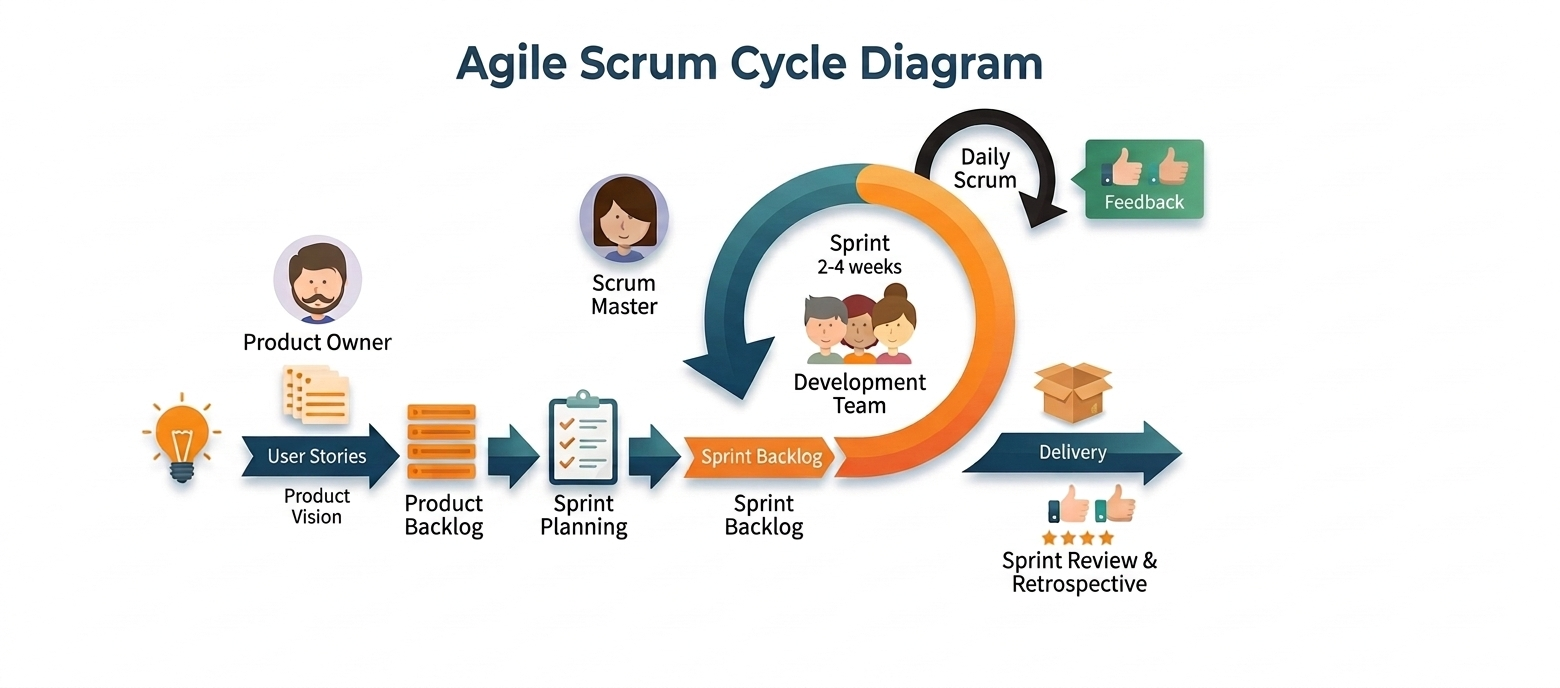
\includegraphics[width=1\columnwidth]{images/scrum_processus.png}
\caption{processus Scrum.}
\label{fig_processus_scrum}
\end{figure}
\subsection{Les avantages de Scrum}
Scrum offre une grande flexibilité et adaptabilité, permettant à l’équipe de s’ajuster rapidement aux changements et aux nouvelles exigences grâce à une approche itérative. Les sprints courts, d’une durée de 2 à 4 semaines, assurent une livraison rapide et continue des fonctionnalités, ce qui facilite l’obtention de retours fréquents des utilisateurs. La transparence et la collaboration sont renforcées par des réunions quotidiennes et des revues de sprint, garantissant que toute l’équipe partage une vision claire de l’avancement du projet. Enfin, Scrum favorise l’amélioration continue grâce aux rétrospectives de sprint, qui permettent d’identifier les points à améliorer et d’optimiser constamment les processus pour accroître la productivité.
\newpage
\subsection{Les acteurs de scrum }
\begin{figure}[htpb]
\centering
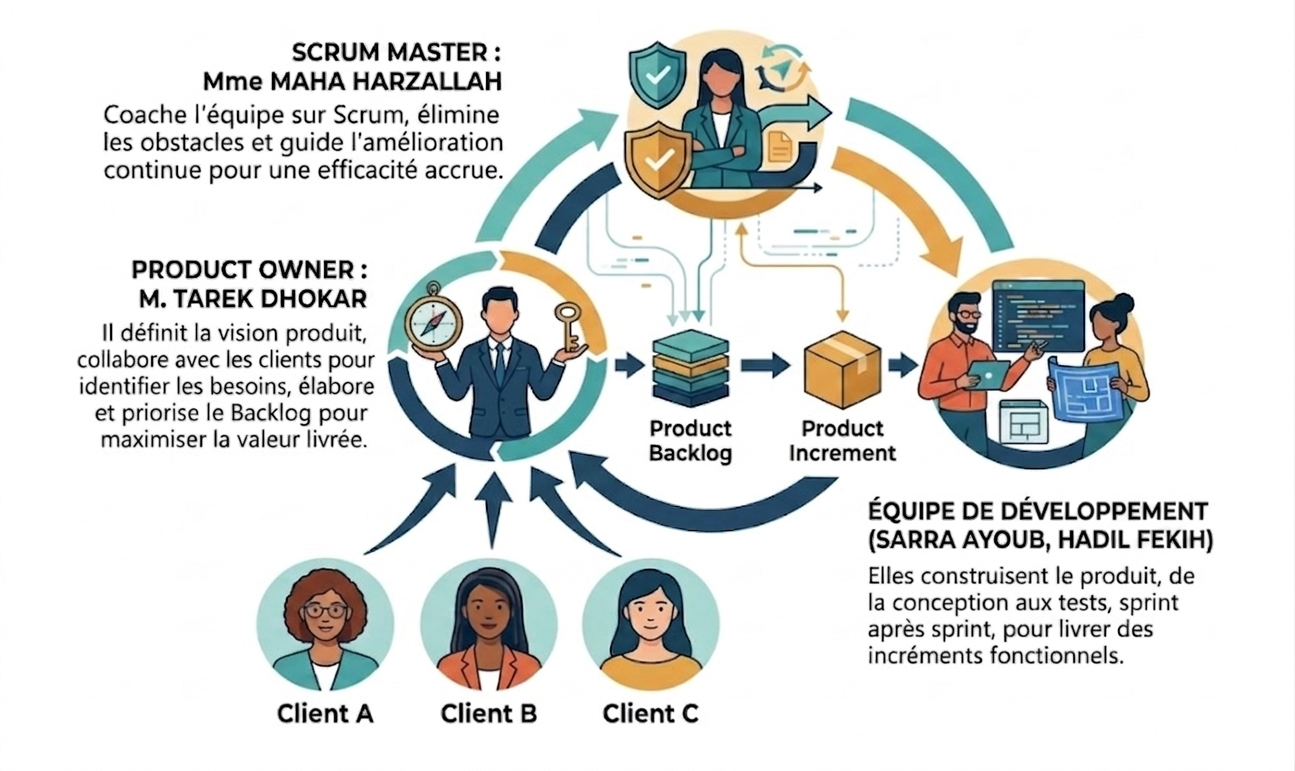
\includegraphics[width=1\columnwidth]{images/arch_scrum.png}
\caption{Les acteurs de scrum.}
\label{fig_precess_scrum}
\end{figure}

\subsection{Les artefacts de Scrum}

Scrum repose sur trois artefacts principaux permettant d’assurer la transparence, le suivi et la progression du projet :
\begin{enumerate}

    \item \textbf{Product Backlog (Backlog Produit)} \\
    Le Product Backlog est une liste ordonnée et évolutive regroupant l’ensemble des fonctionnalités, améliorations et corrections nécessaires au développement du produit. Il est priorisé selon la valeur métier et les besoins des utilisateurs. Sa gestion est assurée par le \textit{Product Owner}, et son contenu est continuellement affiné au fil du projet.

    \item \textbf{Sprint Backlog (Backlog du Sprint)} \\
    Le Sprint Backlog correspond à l’ensemble des éléments sélectionnés du Product Backlog pour être réalisés durant un sprint donné. Il comprend également le plan d’exécution détaillant les tâches nécessaires à leur réalisation. Cet artefact est géré et actualisé par l’équipe de développement tout au long du sprint.

    \item \textbf{Increment (Incrément)} \\
    L’Incrément représente la version fonctionnelle et potentiellement livrable du produit obtenue à la fin de chaque sprint. Il doit satisfaire aux critères définis dans la \textit{Definition of Done} (Définition de Terminé), garantissant le respect des standards de qualité établis par l’équipe.
    
\end{enumerate}
\section{Planification itérative du projet}

Afin d’assurer une organisation efficace du travail, le projet a été structuré en plusieurs sprints conformément à l’approche Agile. Chaque sprint représente une itération limitée dans le temps, avec des objectifs clairement définis et des fonctionnalités précises à réaliser.

Cette planification itérative a permis d’assurer un suivi continu de l’avancement du projet, de prioriser les tâches de manière optimale et d’adapter le développement en fonction des retours obtenus à chaque étape. 

La figure ci-dessous présente la répartition des différentes tâches au sein des sprints.
\begin{figure}[htpb]
    \centering
    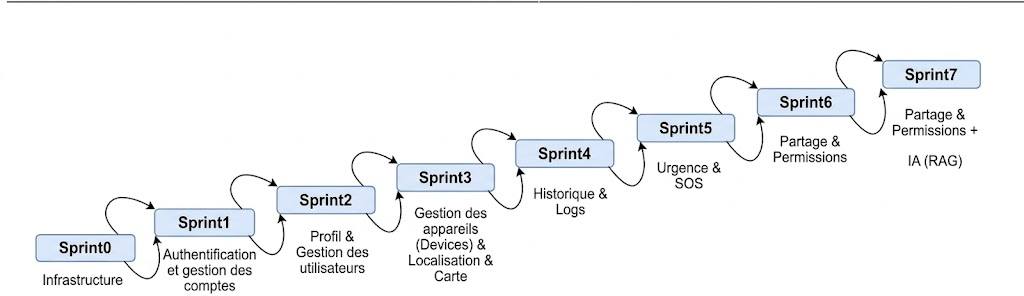
\includegraphics[width=14cm]{images/sprints.jpg}
\end{figure}

% \begin{itemize}
%  \item[$\bullet$ \textbf{Product Owner (PO) :}] « Propriétaire du produit » autrement dit c’est un Business Analyst
% qui représente généralement le client, son rôle est de coordonner un backlog partagé alimentant
% un réseau d’équipes. C’est dans le prochain chapitre que nous montrerons comment nous avons
% incarné le personnage d’un PO pour jouer son rôle et produire notre Backlog Product.
%  \item[$\bullet$ \textbf{Scrum of Scrums Master (SoSM) :}]  C’est le Scrum Master du Scrum of Scrums, responsable
% de la publication des efforts des équipes conjointes.Il doit rendre les progrès visibles. Il travaille
% en étroite collaboration avec plus qu’une équipe scrum pour déployer un incrément de produit
% potentiellement livrable au moins à chaque sprint.
%  \item[$\bullet$ \textbf{ Scrum Master (SM) :}] « Leader de l’équipe Scrum » il est responsable de la supervision
% globale de l’avancement du projet et des activités de l’équipe. Il assure le coaching de l’équipe de
% développement dans des environnements organisationnels. Il organise, tient et planifie également des réunions définies dans Scrum.
%  \item[$\bullet$ \textbf{Dev Team :}] « Équipe de développement » En fait, toute l’équipe Scrum est divisée en groupes
% plus petits, chaque groupe étant composé conventionnellement de trois à neuf membres
% de diverses compétences qui s’engagent à transformer le backlog de produit en incréments de
% fonctionnalités et à élaborer des sprints. Chaque groupe fonctionne comme une équipe Scrum
% indépendante. De plus, chaque équipe choisit une personne - généralement le Scrum Master - qui
% représente l’équipe. Les représentants de chacune des équipes participent aux événements Scrum
% au nom de leur équipe.\\ 
% \end{itemize} 

% En guise de récapitulatif des rôles et de leur distribution au cours de la conduite de notre plateforme CRAWN, Mme Souad DZIRI jouera le rôle du PO, M. Lotfi BEN ROMDHANE jouera le rôle du SoSM,
% M. Lotfi BEN ROMDHANE jouera aussi le rôle du SM de l’équipe 1 du profil génie logiciel (Dev web), M. Lotfi AMMAR
% jouera le rôle du SM de l’équipe 2 des profils cogniticien-mathematicien qui correspondent également à
% l’intelligence artificielle. L’équipe de développement composée de deux groupes sera réduite à une seule personne
% qui est moi-même Wissal FARJALLAH.\\

% Dans l’organigramme \ref{fig_organigramme_sos}, nous proposons de jeter un coup d’oeil à la façon dont la répartition des rôles dans notre environnement Scrum Of Scrums est envisagée

% \begin{figure}[htpb]
% \centering
% 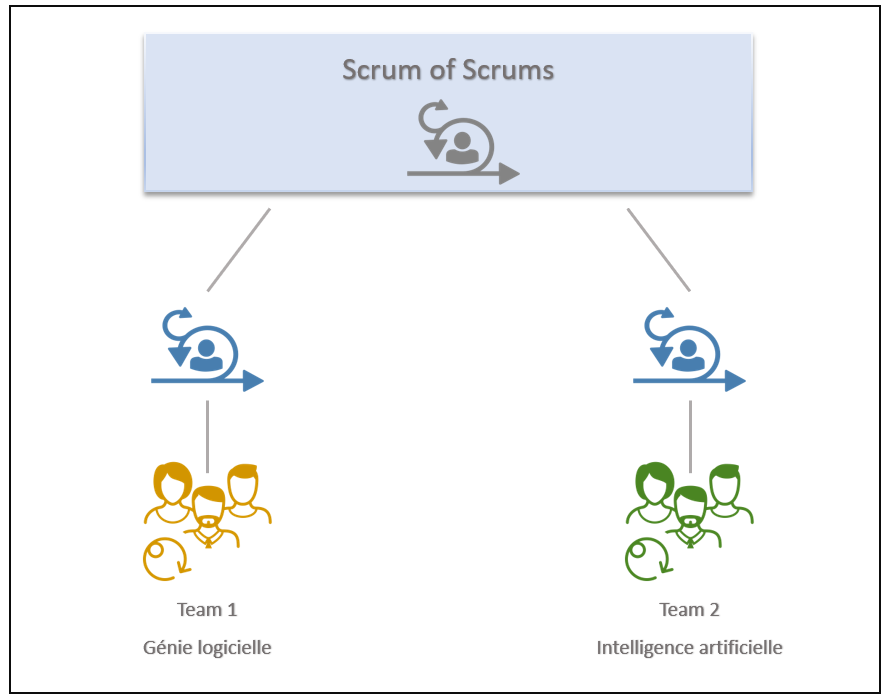
\includegraphics[width=0.9\columnwidth]{images/organigrammeScrum.PNG}
% \caption{Récapitulatif des rôles}
% \label{fig_organigramme_sos}
% \end{figure}
% \newpage
%En tant qu’ingénieure en cours d’apprentissage en phase de stage, j’aurai la précieuse occasion
%de jouer tous ces rôles là. Donc je jouerai le rôle tantôt d’un PO, tantôt d’un SoSM, tantôt d’un SM de
%l’équipe 1, tantôt d’un SM de l’équipe 2 et tantôt de combien de devTeam member de divers profils.
% \subsection{Artefacts dans Scrum of Scrums}
% \begin{itemize}
% \item[$\bullet$ \textbf{Product Backlog (PB) :}] Un Artefact dynamique qui correspond à une liste priorisée des besoins et des exigences du client. Ces besoins sont représentés sous la forme des «Product Backlog items» classés par priorité. C’est le point central de notre projet, qui sera exposé dans
% le chapitre qui suit.

% \item[$\bullet$ \textbf{Sprint Backlog (SB) :}] Est l’ensemble des «Product Backlog items» sélectionnés pour la réalisation de l’objectif du Sprint. C’est une image très visible en temps réel du travail que l’équipe de développement a l’intention d’accomplir pendant le sprint.
% \end{itemize}

% \subsection{Événements dans Scrum of Scrums}
% \begin{itemize}
% \item[$\bullet$ \textbf{Sprint :}]  À l’issue duquel, l’équipe présente un incrément fini potentiellement publiable. Il
% possède un (time-box),avec une durée d’au plus un mois.

% \item[$\bullet$ \textbf{Sprint Planning meeting :}] Le travail à accomplir lors d’un sprint est défini lors de cette
% réunion. Ce plan est élaboré en collaboration avec tous les membres de l’équipe. Selon Scrum
% Guide \cite{scrum}, cette réunion dure au maximum 8 heures pour un sprint d’un mois, 6 heures pour un
% sprint de trois semaines et 4 heures pour un sprint de deux semaines.

% \item[$\bullet$ \textbf{ Stand up Meeting  :}]  Le stand up quotidien Scrum et la réunion quotidienne SoS sont des
% réunions très similaires. Les deux réunions ont pour but de partager l’information, de coordonner
% les activités et d’identifier les problèmes entre les équipes ou entre les membres de l’équipe.

% \item[$\bullet$ \textbf{Sprint Review :}] Se déroulera à la fin de chaque sprint. A ce stade, la Scrum Team et les
% «Stakeholders :les parties prenantes» discutent de ce qui a été réalisé durant le sprint en vue de
% vérifier la qualité de l’incrément potentiellement livrable.

% Remarque : Les Stakeholders peuvent être des (agents bancaires, des experts métier, des experts
% techniques).
% \item[$\bullet$ \textbf{Sprint Retrospective :}] Se déroulera après la revue du sprint. C’est l’occasion pour l’équipe
% Scrum (précisément dans notre cas permettre aux différentes équipes Scrum) de surveiller la
% qualité du processus Scrum, de s’auto-inspecter et de relever les limites identifiées afin de s’améliorer
% lors du prochain Sprint.
% \end{itemize}
% Au fur et à mesure que nous avancerons dans le rapport, nous observerons le dynamisme de la pratique
% du principe SOS.
\section*{Conclusion}
\addcontentsline{toc}{section}{Conclusion}
Ce premier chapitre a permis de présenter le contexte et les objectifs de notre projet, d'analyser les solutions existantes et de définir les exigences pour notre propre solution. Nous avons également présenté la méthodologie de travail que nous avons adoptée pour ce projet, à savoir le framework Scrum, et discuté des avantages de cette approche. Enfin, nous avons introduit le langage de modélisation UML que nous avons utilisé pour la conception de notre application. Dans les chapitres suivants, nous entrerons dans les détails de la conception et du développement de notre solution.